\chapter{Diseño e Implementación de la Propuesta}\label{chapter:design}
El creciente aumento de los datos ha impulsado a que surjan más sistemas AutoML. Estos han demostrado que en gran medida disminuyen 
el desgaste de los científicos de datos en tareas que requieran mucho tiempo y que sean engorrosas de realizar. También aceleran 
el proceso de predicción y en los ensayos realizados sobre los mismos han confirmado ser bastante eficientes. En aras de justificar 
su correcto funcionamiento, los benchmark han sido una pieza esencial(Ver capítulo 1).

Cada uno de estos sistemas de prueba siguen estrategias para seleccionar sus conjuntos, la métrica y el tiempo, los cuales permiten 
comparar y medir el rendimiento de una herramienta de aprendizaje automático. En el capítulo 1 se realizó un estudio exhaustivo 
sobre los benchmark presentes en la literatura. Como bien se explicó, cada uno tuvo su aporte, ya que en el momento de su creación 
permitieron validar la eficiencia de los sistemas. A pesar de este, producto al avance y evolución de muchos de estos softwares y a 
la aparición de otros nuevos, dichas pruebas han pasado a ser obsoletas. Además de que algunas, hasta las más actuales, tuvieron 
fallas en su metodología de creación, lo cual tronchó el cumplimiento de sus objetivos principales. También el dominio y 
la estructura de los datos ha pasado desapercibido para cada uno de estos. El dominio tabular han sido el protagonista, 
así como los datos estructurados y procesados, y está claro que estos son los menos abundantes en el mundo.

Debido a la ineficacia y errores de los anteriores benchmarks para medir el rendimiento de los actuales sistemas AutoML se propuso 
crear uno nuevo llamado \textbf{HAutoML-Bench}. La meta es verificar la flexibilidad de los sistemas AutoML ante diferentes tipos de entrada, 
diferentes dominios y distintas tareas. También validar su heterogeneidad viendo si permiten enfrentarse a problemas reales en donde 
los datos se encuentran sin mucho procesamiento.

\section{Metodología del Diseño }\label{section:design}

Las características principales que definieron la metodología del diseño de \textbf{HAutoMLBench} fueron los conjuntos de datos y las métricas de 
rendimiento que permitieron realizar una experimentación con los mismos. Sobre los conjuntos fue necesario definir su estrategia de selección,
forma de división y problemas que surgieron durante su procesamiento.

\begin{flushleft} 
    {\large { \textbf{Estrategias de selección del conjunto de Datos del Benchmark}}}\label{section:selection}
\end{flushleft}
La selección de los conjuntos de datos determina la vertiente a la que va dirigida la evaluación de los sistemas. Estos deben ser los encargados de someter con 
pruebas complicadas al software evaluado en aras de resaltar las buenas y las malas funcionalidades del mismo.

Para cumplir con lo anteriormente planteado en este benchmark se buscaron problemas difíciles, semejantes a los de la vida real y en donde el dominio de los datos 
sea importante. Para ello, de sitios como Hungging Face, Kaggle, Iberle se escogieron 26 conjuntos: 16 son de dominio texto puro y 10 son multimodales. Se decidió 
incluir datasets multimodales porque en la vida real los datos no se encuentran separados por dominios, estos tienden a coexistir. Los conjuntos se encuentran 
representados en tablas, pero aun así presentan su semántica, ya que ninguna de sus columnas internas fueron procesadas y son linealmente independientes. Cada una de 
estas continúan teniendo su significado y estructura original relacionado con el dominio al que pertenecen.

En el dominio texto puro se buscó diversidad respecto a tener como tipo de entrada documentos, oraciones, palabras. El solo tratar con una entrada de texto requiere 
técnicas de procesamiento especializadas por parte de los sistemas, se decidió agregar aquellos que tuvieran una y más. Existen conjuntos en idioma español y en inglés, 
uno es multilingual.

Con respecto a los multimodales forman parte algunos presentes en el benchmark (Text Multimodal), solo se utilizó su referencia original porque en este los conjuntos 
fueron procesados, lo que se desvía del objetivo principal de \textbf{HAutoML-Bench}. Respecto a las columnas corresponden a texto, oraciones, palabras, columnas categóricas, 
booleanas, valores numéricos tanto discretos como continuos, columnas de tiempo y que responden a urls de páginas y de imágenes.

A modo general se buscó incluir conjuntos de datos que tuvieran valores faltantes y desequilibrio de clases, ya que como se dejó claro en (Cap1) suelen ser 
características que son un desafío. Respecto al ambiente de aplicación forman parte datasets relacionados con el fraude, a la medicina, problemas sociales. Algunas de 
las tareas que resuelven requieren técnicas de análisis de sentimientos, búsqueda de similitud entre texto, oraciones, identificación del lenguaje, interpretación, 
análisis de series temporales. Todas las tareas presenten se reducen a una clasificación binaria, multiclase, regresión o reconocimiento de entidades.

Luego, para continuar en búsqueda de más diversidad y tratar de no caer en sesgos en la selección, se buscaron datasets de diferente número de instancias en el rango 
de los cientos, miles, 10 miles y 100 miles. También variedad en el número de columnas y de clases. Además, en la forma en que se modelan las salidas ejemplo, la 
clasificación puede darse a través de valores numéricos o de etiquetas que representen las categorías. En la tabla (tal) puede verse las características que cumple 
cada datasets.
\begin{flushleft} 
    {\large { \textbf{Método de división de los Conjuntos}}}\label{section:division}
\end{flushleft}
La mayoría de los benchmark vistos en el capítulo 1 utilizaron validación k-fold como método de evaluación, dividiendo de forma 
aleatoria en cada prueba los conjuntos en entrenamiento y validación. HAutoMLBench provee un conjunto de entrenamiento y un conjunto de prueba (método hold hot). 
Se utililizó esa forma debido a que muchos de los datasets originales estaban previamente divididos así por reglas del dominio al que pertenecen. 
Además de que cross-validation resulta ser mas costoso y evaluar en un conjunto de datos nunca antes visto resultó una mejor opción.  

Otros estaban separados en entrenamiento, validación y test, para este caso se 
tomaron varias estrategias. Para paws-x-es, paws-x-es, wikineural-es y wikineural-en se unieron validación con prueba, ya que los datos de entrenamiento era 
demasiado grande en comparación con la unión de prueba con validación. Los restantes se unieron validación y entrenamiento. Aquellos datasets que no se encontraban 
divididos en partes, en dependencia de su tamaño, se escogió entre el 80 y 70 porciento para entrenamiento y lo restante para prueba. En la tabla se muestran 
los resultados de las divisiones realizadas. 

Se decidió optar por la estrategia de división antes descrita en lugar de entrenamiento - validación-prueba, ya que 
todos los sistemas no permiten como entrada la división del conjunto de entrenamiento. Además, es interés de este benchmark que todos los sistemas exploten todas sus 
funcionalidades. Entre estas está la división del conjunto de entrenamiento.

\begin{flushleft} 
    {\large { \textbf{Problemas en los Conjuntos de Datos}}}\label{section:dataproblems}
\end{flushleft}
Los conjuntos de datos originales escogidos tenían una estructura y un formato bastante asequible y entendible. Sin embargo, algunos sufrieron ciertas transformaciones 
para convertirse en los datasets oficiales del benchmark debido a ciertos problemas. Los más sobresalientes fueron en texto, 
problemas con caracteres corruptos, los cuales fueron eliminados o sustituidos por su igual sin corromper. También falta de los delimitadores que llevaron a utilizar 
otras técnicas de lectura en vez de las propias del tipo de archivo a leer.


\begin{flushleft} 
    {\large { \textbf{Métricas de Rendimiento}}}\label{section:metrics}
\end{flushleft}
En ocasiones suele confundirse la métrica con la función de pérdida. La función de pérdida es una forma de medir el rendimiento del modelo durante el 
entrenamiento. Las métricas se utilizan para juzgar y cuantificar los resultados luego de este. En el caso de los sistemas AutoML la métrica suele usarse 
durante el entrenamiento. Esta suele tener dos funcionalidades: optimización y evaluación. La primera se encarga de actualizar los pesos de los modelos durante el 
entrenamiento en el proceso de validación. La segunda permite obtener características del rendimiento en conjunto de datos nunca antes visto por el sistema durante 
la evaluación.

Es ideal que la misma métrica que se utilice para optimizar se utilice en una evaluación para validar la eficiencia del sistema. También es cierto que muchos conjuntos 
de datos para su entendimiento necesitan evaluarse en más de una métrica. Debido a lo anteriormente planteado, se seleccionaron un conjunto de métricas por tipo de 
tarea, cualquiera puede usarse para la optimización, ya que todas serán medidas durante el proceso de evaluación.

La tarea clasificación se evalúa en accuracy, balanced-accuracy, precisión, recall y f1.  En la clasificación binaria para las tres últimas se utiliza tanto su versión 
normal como la micro y en la multiclase la macro y la weighted. Para la regresión rmse, mse, mae. En tareas de entidades y relaciones . Aún no sé cuál usar 
La selección de métrica de optimización quedó libre debido a que esta es dependiente del AutoML evaluado, muchos de estos no las implementan todas o 
restringen sus modelos a unas específicas. Se recomienda usar para clasificación balanced-accuracy debido a que existe un gran desequilibrio en algunos de 
los conjuntos de datos que modelan este tipo de tarea, mientras que para la regresión rmse que permite una interpretación directa con el error entre el resultado 
predictivo y el verdadero.

\section{Detalles de Implementación}\label{section:Implementation}
\textbf{HAutoML-Bench} es un sistema extensible , de código abierto y que aún continúa en desarrollo. Permite la descarga de datasets y la incluisión de otros. 
Además contiene funcionalidades para cuantificar el rendimieto en los mismos y para filtarlos según sus metadatos.

\begin{flushleft} 
    {\large { \textbf{ Instrucciones de Instalación e Inicialización}}}\label{section:instructions}
\end{flushleft}

 
\begin{itemize}
    \item Para su instalación solo es necesario descargarlo desde su repositorio oficial de github. 
    \item Instalar poetry un gestor de paquetes.   
    \item instalar todas las dependencias del benchmark con el comando ¨poetry install¨.
    \item Luego debe colocar el archivo en donde va a realizar las pruebas en la carpeta source e importar la clase HAutoML-Bench
    \item LLamar al metodo create de la siguiente forma HAutoML-Bench.create(). 
\end{itemize}
\begin{flushleft} 
    {\large { \textbf{Estructura del software}}}\label{section:struct}
\end{flushleft}


\textbf{HAutoML-Bench} está formado por dos clases la clase HAutoMLBench y clase Dataset. En la figura \ref{fig:image1} se muestra la estructura de sus archivos inicialmente.
En el directorio source archivo test se provee algunos ejemplos de uso del benchmark para su fácil utilizacion.

\begin{figure}[H]
    \centering
    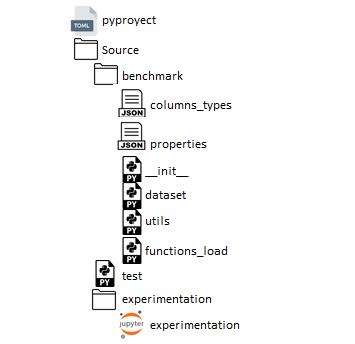
\includegraphics[width=0.5\textwidth]{Graphics/directory.png}
    \caption{Directorio del Benchmark}
    \label{fig:image1}
 \end{figure}

\begin{flushleft} 
    {\large { \textbf{ Clase Benchamrk y Dataset}}}\label{section:class}
\end{flushleft}

La clase HAutoMLBench es la encargada de interactuar con el usuario , en ella están los métodos que el usuario debe utilizar para 
probar sus sistemas. Estos son estáticos de tal forma que no se necesite instanciar la clase para utilizar sus funcionalidades.

La clase dataset modela las propiedades de un dataset: información,nombre, url utilizada para su descarga y función load.

\begin{flushleft} 
    {\large { \textbf{ Metodos de interaccion del usuario }}}\label{section:methods}
\end{flushleft}


El método create'datasets como se mencionó anteriormente en las instruccionde de instalación es el encargado de crear los archivos que guardan el estado del benchmark
, almacena los nombres de los datsets registrados así como su ur, nombre de la función load y sus información propia. Además se encarga de crear las intancias de los dastasets y 
serializarlas para su futuro uso. Es importante que solo se ejecute esta función una sola vez debido a que perderá todos los cambios guardados y volverá a su estado inicial por defecto.
En la figura \ref{fig:image2} se muestra el flujo de ejecución de la función. 

\begin{flushleft} 
    { \textbf{ Método create-datasets }}\label{section:create}
\end{flushleft}

\begin{figure}[H]
    \centering
    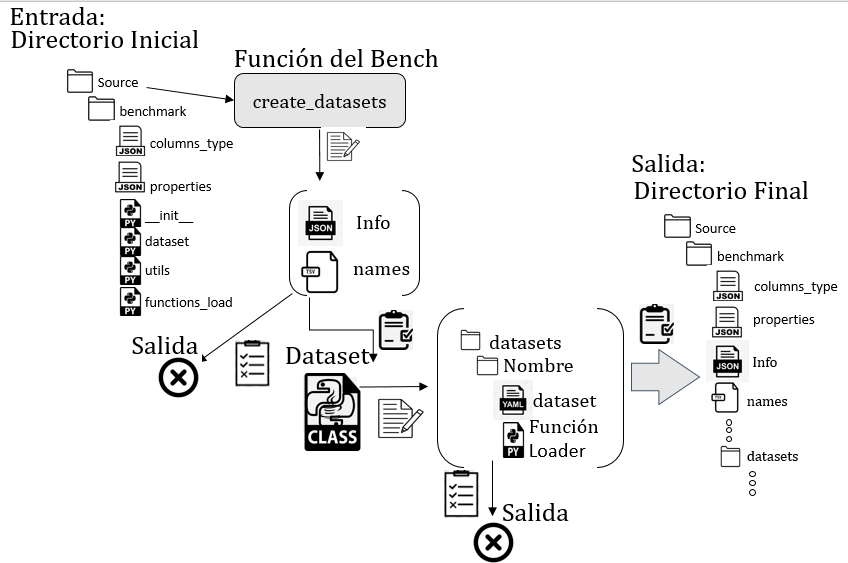
\includegraphics[width=0.9\textwidth]{Graphics/methods/create-datasets.png}
    \caption{Flujo de trabajo: Método create-datasets}
    \label{fig:image2}
 \end{figure}

\begin{flushleft} 
    { \textbf{Método init }}\label{section:init}
\end{flushleft}

 \begin{figure}[H]
    \centering
    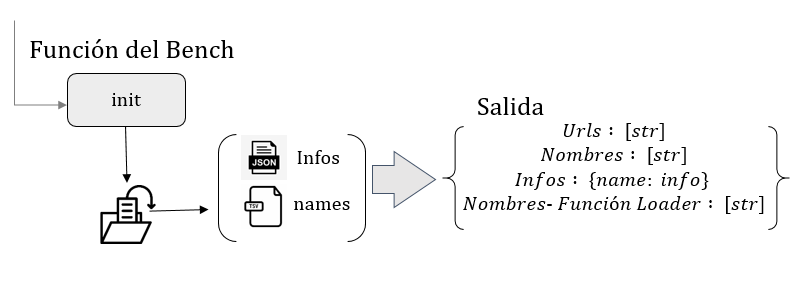
\includegraphics[width=0.9\textwidth]{Graphics/methods/init.png}
    \caption{Flujo de trabajo: Método init}
    \label{fig:image2}
 \end{figure}

\begin{flushleft} 
    { \textbf{Método new-dataset }}\label{section:new}
\end{flushleft}

 \begin{figure}[H]
    \centering
    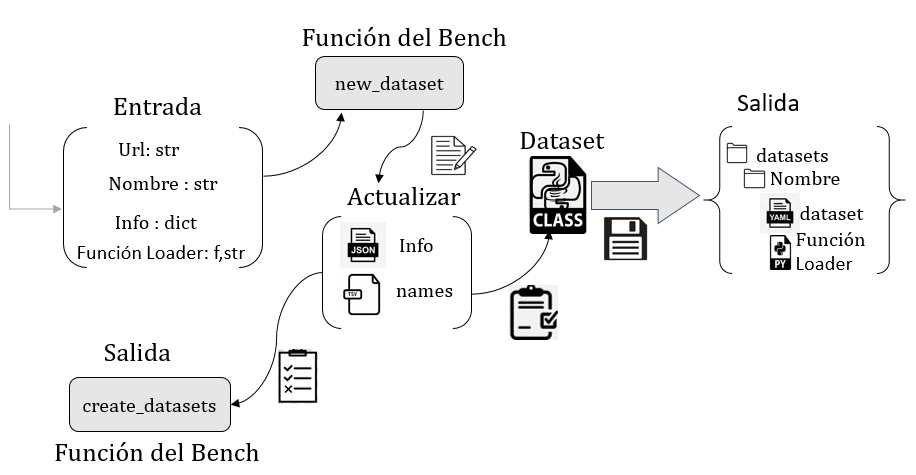
\includegraphics[width=0.9\textwidth]{Graphics/methods/new-dataset.png}
    \caption{Flujo de trabajo: Método new-dataset}
    \label{fig:image3}
 \end{figure}

 
\begin{flushleft} 
    { \textbf{Método remove-dataset }}\label{section:remove}
\end{flushleft}

 \begin{figure}[H]
    \centering
    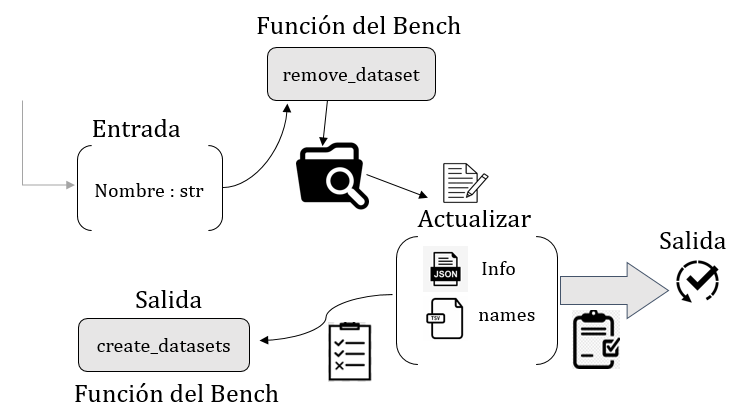
\includegraphics[width=0.9\textwidth]{Graphics/methods/remove-dataset.png}
    \caption{Flujo de trabajo: Método remove-dataset}
    \label{fig:image4}
 \end{figure}

\begin{flushleft} 
    { \textbf{Método load-dataset }}\label{section:load_d}
\end{flushleft}

 \begin{figure}[H]
    \centering
    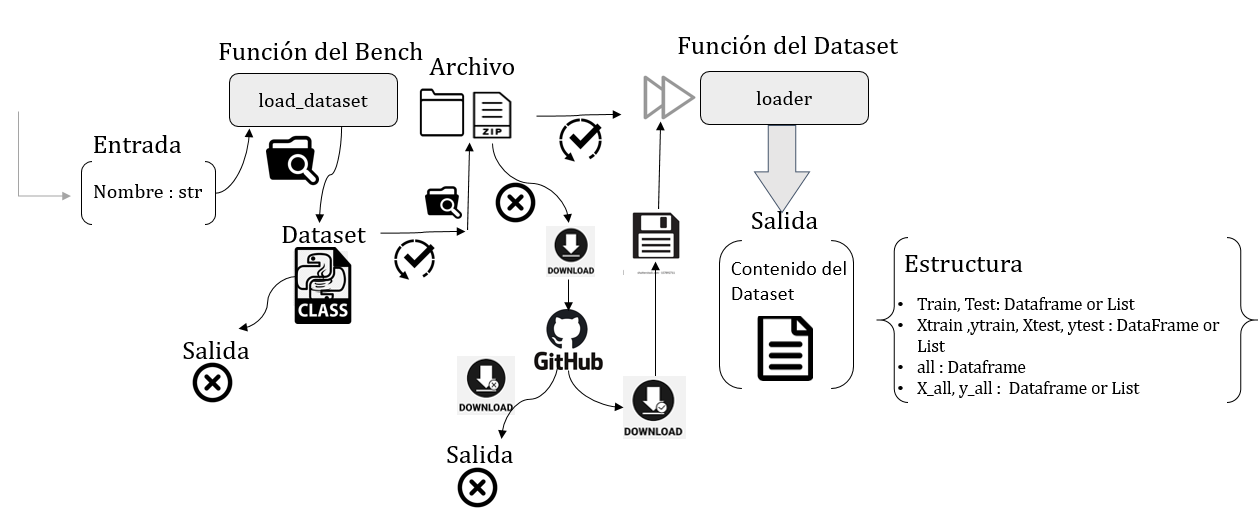
\includegraphics[width=1 \textwidth]{Graphics/methods/load-dataset.png}
    \caption{Flujo de trabajo: load-dataset}
    \label{fig:image5}
 \end{figure}

\begin{flushleft} 
    { \textbf{Método load-info }}\label{section:load_i}
\end{flushleft}

 \begin{figure}[H]
    \centering
    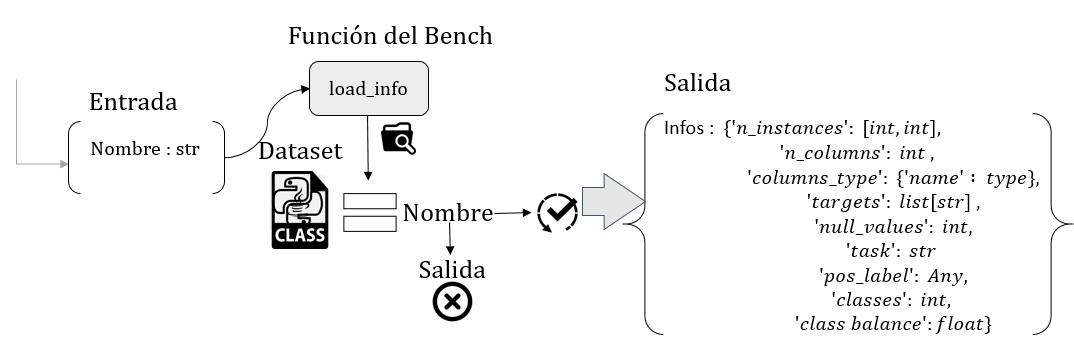
\includegraphics[width= 0.9\textwidth]{Graphics/methods/load_info.png}
    \caption{Flujo de trabajo: load-info}
    \label{fig:image6}
 \end{figure}

\begin{flushleft} 
    { \textbf{Método filter }}\label{section:filter}
\end{flushleft}

 \begin{figure}[H]
    \centering
    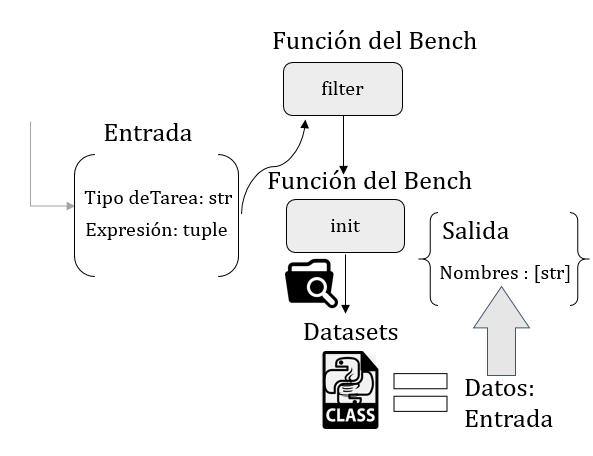
\includegraphics[width=0.8\textwidth]{Graphics/methods/filter.png}
    \caption{Flujo de trabajo: Método filter}
    \label{fig:image7}
 \end{figure}


metodos auxiliares









